
\documentclass[11pt]{article}

% Paquetes
%===================================================================================================

% Establecemos los márgenes
\usepackage[a4paper, margin=1in]{geometry}

% Separacion entre parrafos
\setlength{\parskip}{1em}

% Paquete para incluir codigo
\usepackage{listings}

% Paquete para incluir imagenes
\usepackage{graphicx}
\graphicspath{ {./images/} }

% Para fijar las imagenes en la posicion deseada
\usepackage{float}

% Para que el codigo acepte caracteres en utf8
\lstset{literate=
  {á}{{\'a}}1 {é}{{\'e}}1 {í}{{\'i}}1 {ó}{{\'o}}1 {ú}{{\'u}}1
  {Á}{{\'A}}1 {É}{{\'E}}1 {Í}{{\'I}}1 {Ó}{{\'O}}1 {Ú}{{\'U}}1
  {à}{{\`a}}1 {è}{{\`e}}1 {ì}{{\`i}}1 {ò}{{\`o}}1 {ù}{{\`u}}1
  {À}{{\`A}}1 {È}{{\'E}}1 {Ì}{{\`I}}1 {Ò}{{\`O}}1 {Ù}{{\`U}}1
  {ä}{{\"a}}1 {ë}{{\"e}}1 {ï}{{\"i}}1 {ö}{{\"o}}1 {ü}{{\"u}}1
  {Ä}{{\"A}}1 {Ë}{{\"E}}1 {Ï}{{\"I}}1 {Ö}{{\"O}}1 {Ü}{{\"U}}1
  {â}{{\^a}}1 {ê}{{\^e}}1 {î}{{\^i}}1 {ô}{{\^o}}1 {û}{{\^u}}1
  {Â}{{\^A}}1 {Ê}{{\^E}}1 {Î}{{\^I}}1 {Ô}{{\^O}}1 {Û}{{\^U}}1
  {ã}{{\~a}}1 {ẽ}{{\~e}}1 {ĩ}{{\~i}}1 {õ}{{\~o}}1 {ũ}{{\~u}}1
  {Ã}{{\~A}}1 {Ẽ}{{\~E}}1 {Ĩ}{{\~I}}1 {Õ}{{\~O}}1 {Ũ}{{\~U}}1
  {œ}{{\oe}}1 {Œ}{{\OE}}1 {æ}{{\ae}}1 {Æ}{{\AE}}1 {ß}{{\ss}}1
  {ű}{{\H{u}}}1 {Ű}{{\H{U}}}1 {ő}{{\H{o}}}1 {Ő}{{\H{O}}}1
  {ç}{{\c c}}1 {Ç}{{\c C}}1 {ø}{{\o}}1 {å}{{\r a}}1 {Å}{{\r A}}1
  {€}{{\euro}}1 {£}{{\pounds}}1 {«}{{\guillemotleft}}1
  {»}{{\guillemotright}}1 {ñ}{{\~n}}1 {Ñ}{{\~N}}1 {¿}{{?`}}1 {¡}{{!`}}1
}

% Para que no se salgan las lineas de codigo
% Para fijar una fuente que resalte
\lstset{breaklines=true, basicstyle=\ttfamily}

% Para que los metadatos que escribe latex esten en español
\usepackage[spanish]{babel}
\decimalpoint % Para que no se cambie el punto a la coma

% Para la bibliografia
% Sin esto, los enlaces de la bibliografia dan un error de compilacion
\usepackage{url}

% Para que se puedan clicar los enlaces
\usepackage{hyperref}

% Para mostrar graficas de dos imagenes, cada una con su caption, y con un caption comun
\usepackage{subcaption}

% Simbolo de los numeros reales
\usepackage{amssymb}

% Para que los codigos tengan una fuente distinta
\usepackage{courier}

\lstdefinestyle{CustomStyle}{
  language=Python,
  numbers=left,
  stepnumber=1,
  numbersep=10pt,
  tabsize=4,
  showspaces=false,
  showstringspaces=false
  basicstyle=\tiny\ttfamily,
}

% Para referenciar secciones usando el nombre de las secciones
\usepackage{nameref}

% Para enumerados dentro de enumerados
\usepackage{enumitem}

% Para mejores tablas
\usepackage{tabularx}

% Para poder tener el mismo identificador en dos tablas separadas
\usepackage{caption}

% Mostrar la página de las referencias en el indice del documento
\usepackage[nottoc,numbib]{tocbibind}

% Para mostrar las matrices
\usepackage{amsmath}

% Para que las notas al pie de pagina queden bien abajo
\usepackage[bottom]{footmisc}

% Para poner tablas en horizontal, ocupando bien la página
% cuando hay mucho texto en la table
\usepackage{lscape}

% Comandos personalizados
%===================================================================================================
% Here all custom commands are defined

% Para realizar las citas de forma corta
\newcommand{\customcite}[1]{\emph{"\ref{#1}. \nameref{#1}"}}

% Para entrecomillar un texto
\newcommand{\entrecomillado}[1]{\emph{``#1''}}




% Metadatos del documento
%===================================================================================================
\title{
    Estudio sobre la empleabilidad de los estudiantes
}

\author{
    {Sergio Quijano Rey}\\
    {sergioquijano@correo.ugr.es}
}

\date{\today}

% Separacion entre parrafos
\setlength{\parskip}{1em}

% Contenido del documento
%===================================================================================================
\begin{document}

% Portada del documento
\maketitle
\pagebreak

% Indice de contenidos
\tableofcontents

% Lista de figuras
% Uso el addtocontents para que no se muestre la seccion de indice de figuras en el indice inicial

\addtocontents{toc}{\setcounter{tocdepth}{-10}}
\listoffigures

\listoftables

% \lstlistoflistings
\addtocontents{toc}{\setcounter{tocdepth}{3}}

\pagebreak

% Contents of the document

\section{Abstract}

En este trabajo, estudiaremos una base de datos consistente en métricas recogidas durante entrevistas de prueba, junto a si los candidatos son o no escogidos para el hipotético puesto de trabajo.

Con \textbf{dos objetivos} en mente:

\begin{itemize}
    \item Construir un clasificador eficiente para predecir la empleabilidad
    \item Usar la base de datos para realizar un estudio sobre lo meritocrático del proceso. Dicho experimento consiste en entrenar dos modelos, uno usando las variables que consideramos meritocráticas, y otro usando las variables que consideramos no meritocráticas. Si el modelo que usa variables no meritocráticas funciona mejor, podemos pensar que entonces el proceso de selección se basa más en estos aspectos, que hemos considerado no meritocráticos
\end{itemize}

Para ello, realizaremos:

\begin{itemize}
    \item Un estudio univariante de la base de datos, destacando el tratamiento de \textit{outliers}, el estudio de la normalidad univariante, y un análisis descriptivo clásico
    \item Un estudio multivariante de la base de datos, destacando el estudio de las correlaciones entre variables, tratamiento multivariante de \textit{outliers}, estudio de normalidad multivariante y reducción de la dimensionalidad con \textit{PCA} y \textit{FA}
    \item Ajuste de los modelos, destacando una pequeña exploración de hiperparámetros, entrenamiento y validación, comparando los resultados
    \item El experimento adicional, previamente mencionado
\end{itemize}

Al final, conseguimos obtener un modelo muy robusto a la hora de realizar predicciones, y todo el análisis realizado en el cuaderno, más el experimento adicional, confirman de forma contundente la falta de meritocracia en el proceso de selección.




\newpage

\section{introduccion}

TODO


% TODO -- Último párrafo diciendo cuáles han sido los objetivos del trabajo
% TODO -- Le da relevancia a que comentemos el estado del arte
% TODO -- Importancia a referencias a otros trabajos

\newpage

\section{materialesmetodos}

TODO


% TODO -- Describir la base de datos que usamos
% TODO -- Los métodos no deben ser más de 400 palabras, describiendo los métodos estadísticos que hemos usado

TODO -- comentar que la base de datos usada se encuentra en \cite{database:online}


\subsection{Materiales}

En primer lugar, la \textbf{base de datos se puede obtener} del repositorio de \textit{Kaggle} \cite{database:online}.

Como ya se ha comentado previamente, la base de datos se compone de registros con métricas de candidatos en entrevistas de trabajo de pruebas (para entrenar a los candidatos en estas entrevistas), junto con si el candidato es escogido o no para el hipotético puesto de trabajo.

El conjunto de datos se compone originalmente de 10 columnas (variables) y 2983 filas (registros). Las variables que contiene la base de datos son las siguientes:

\begin{enumerate}
    \item Identificador numérico del estudiante. Lo llaman nombre del estudiante, pero en verdad se corresponde con una etiqueta numérica del tipo \entrecomillado{Student \textless id \textgreater}
    \item Apariencia general
    \item Formas de hablar
    \item Condición física
    \item Agilidad mental
    \item Confianza en si mismo
    \item Habilidad para presentar ideas
    \item Habilidades de comunicación
    \item Rendimiento académico
    \item Empleabilidad
\end{enumerate}

Todas las variables, salvo el identificador y la empleabilidad, son variables discretas tomando valores del 1 al 5. La estructura del identificador ya la hemos comentado. Y la empleabilidad toma dos valores de tipo \textit{string}: empleable o no empleable.

En \cite{database:online}, se comenta que la base de datos no ha sido tratada de ningún modo. Sin embargo, podemos inspeccionar la base de datos manualmente. El identificador llega hasta un valor de 3000, pero solo tenemos 2983 filas. Como vemos más adelante, no tenemos valores faltantes, así que asumimos con bastante seguridad que las 17 filas que faltan tenían valores faltantes, y se han borrado.

No usamos para nada el identificador del estudiante, así que de ahora en adelante, nos podemos olvidar de esa variable. Mostramos ahora algunos estadísticos básicos sobre el conjunto de datos sin tratar:

\begin{table}[H]
\scalebox{0.8}{
\begin{tabular}{lllllllll}
    Variable &  Mínimo & Máximo & 1º Cuartil  & Media & Mediana & 3º Cuartil & Desv. Típica \\
    \hline
    Agilidad mental & 2.0 & 5.0 & 3.0 & 3.963 & 4.0 & 5.0 & 0.7814509 \\
    Rendimiento académico & 3.0 & 5.0 & 4.0 & 4.611 & 5.0 & 5.0 & 0.6895586 \\
    Formas de hablar & 2.0 & 5.0 & 3.0 & 3.885 & 4.0 & 4.0 & 0.7527855 \\
    Condición física & 2.0  & 5.0  & 3.0  & 3.972  & 4.0  & 5.0 & 0.7466378 \\
    Apariencia & 2.0 & 5.0 & 4.0 & 4.247 & 4.0 & 5.0 & 0.6824864 \\
    Confianza & 2.0 & 5.0 & 3.0 & 3.911 & 4.0 & 5.0 & 0.8074833\\
    Habilidad para presentar ideas & 2.0 & 5.0 & 3.0 & 3.814 & 4.0 & 4.0 & 0.7339429 \\
    Habilidades comunicativas & 2.0 & 5.0 & 3.0 & 3.525 & 3.0 & 4.0 & 0.7371541 \\

\end{tabular}
}
\caption{Resumen del conjunto de datos original}
\end{table}

Con esto vemos que aunque las métricas van, en un diseño inicial, del valor 1 al 5, muchas de ellas tienen un rango más acotado (por debajo), puesto que no hubo participantes que obtuviesen los valores mínimos.

Al estar trabajando con variables discretas, el siguiente gráfico es muy útil a la hora de visualizar la distribución de los datos:

\begin{figure}[H]
    \centering
    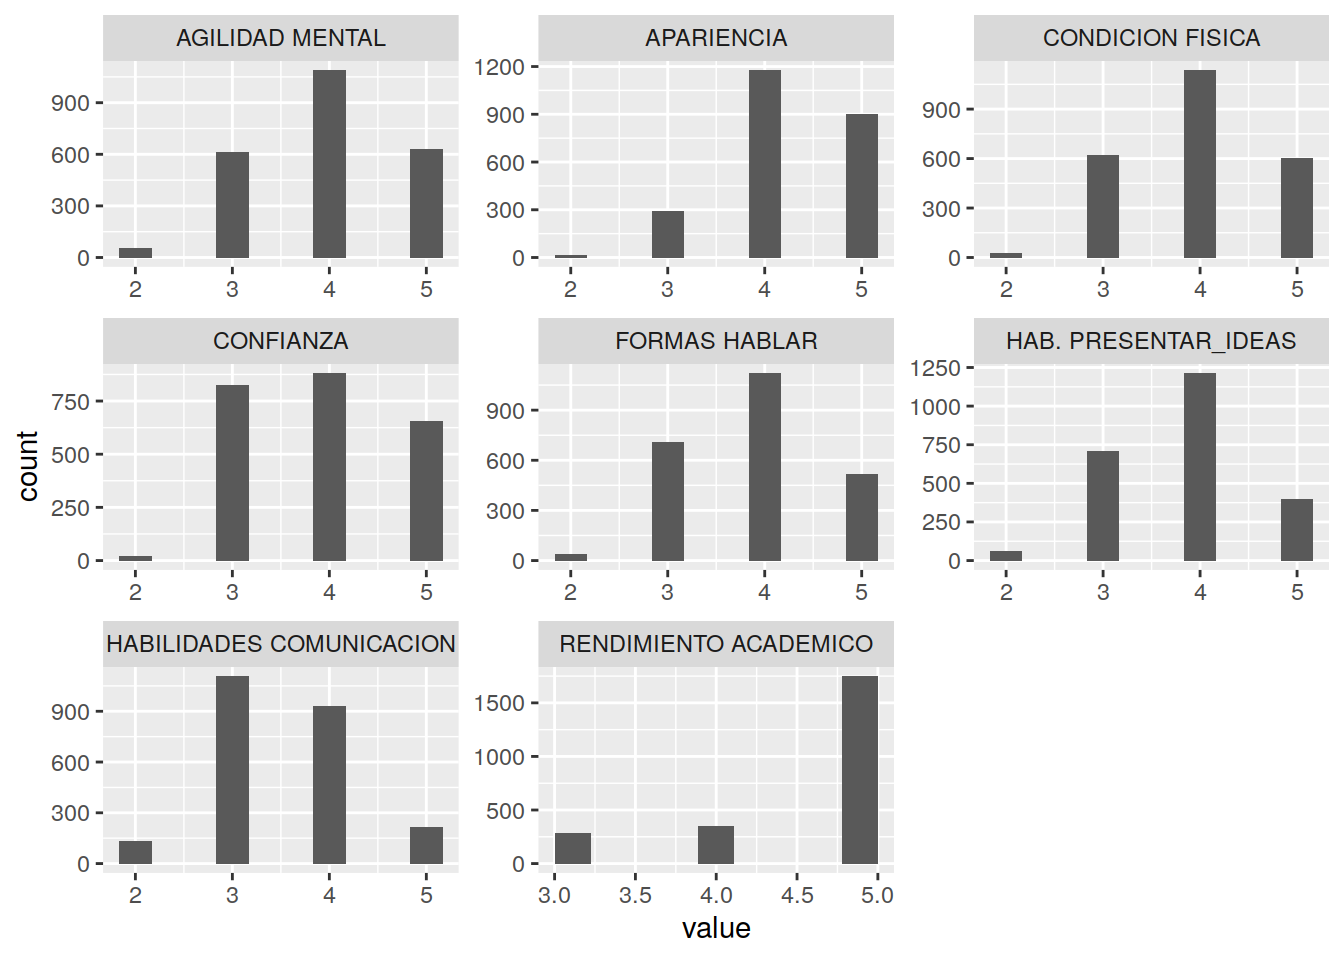
\includegraphics[width=0.8\textwidth]{histogramas_variables}
    \caption{Histograma de las variables de entrada}
\end{figure}

Mostramos gráficamente la distribución de la variable de salida:

\begin{figure}[H]
    \centering
    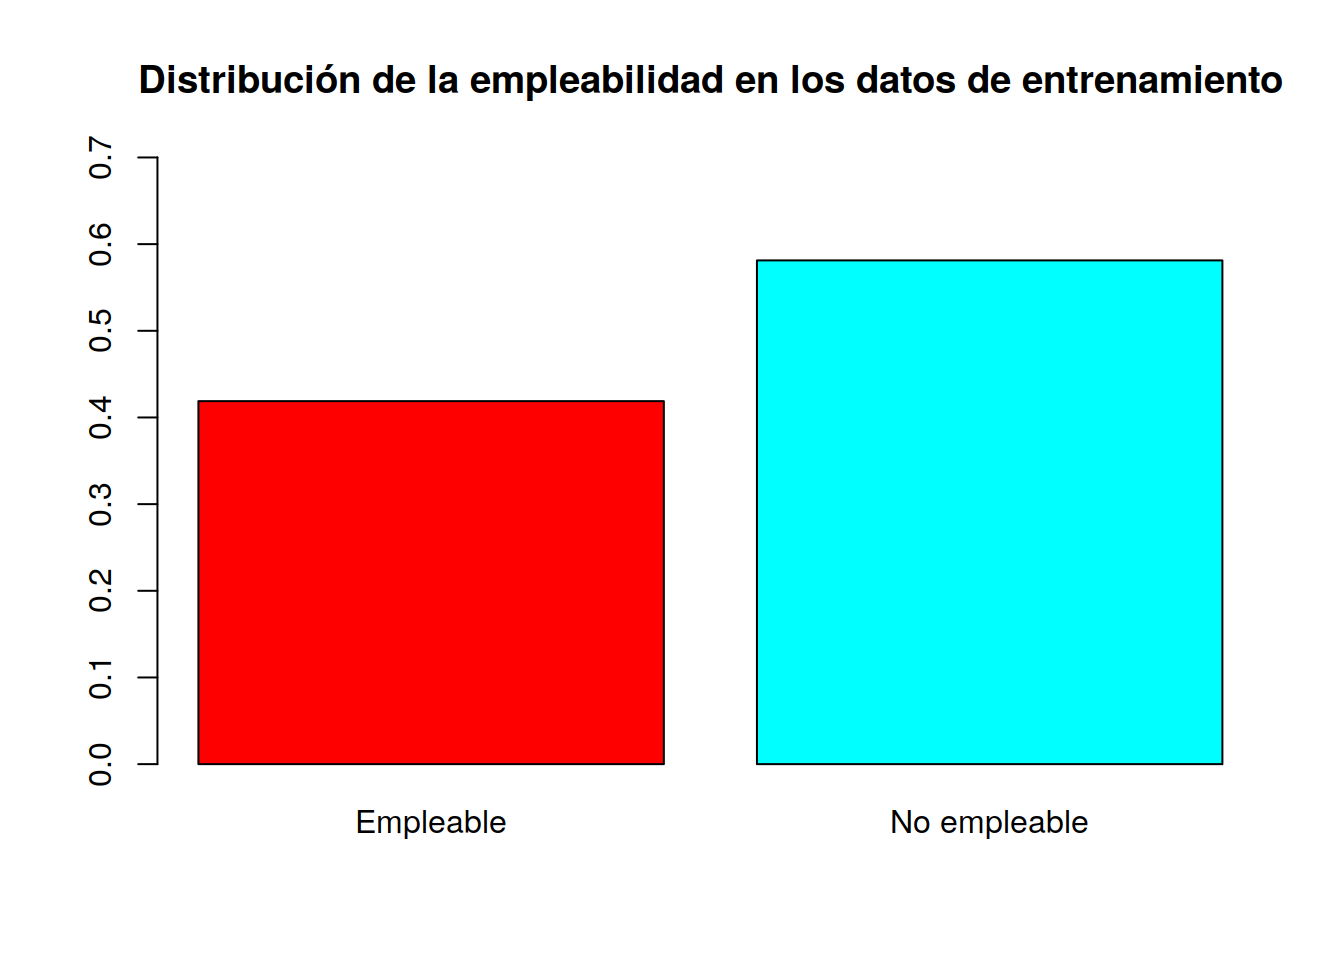
\includegraphics[width=0.6\textwidth]{balanceo_clases}
    \caption{Distribución de la variable de salida, con la que podemos estudiar el balanceo de las clases}
\end{figure}


Hay cierto desbalanceo hacia la no empleabilidad, aproximadamente un $40-60\%$. De normal, este desbalanceo no es demasiado grave. Además, considerando el desbalanceo esperable dado el contexto en el que estamos (un porcentaje mayoritario no debería ser aceptado para un trabajo), consideramos que no necesitamos aplicar alguna técnica para tratar este desbalanceo (i.e. podría aplicarse \textit{SMOTE}).

\subsection{Métodos}


% TODO -- Los métodos no deben ser más de 400 palabras, describiendo los métodos estadísticos que hemos usado

\newpage

\section{Resultados}



\newpage

\section{discusion} \label{section:Discusion}

TODO


% TODO -- Comentar, interpretar y explicar lo que significan los resultados

\newpage

\section{conclusion}

TODO

\newpage

\pagebreak


% Which style to use to show references
\bibliographystyle{ieeetr}

% Show the references
\bibliography{./References}

\end{document}
